\documentclass{beamer}

% Theme selection
\usetheme{Madrid}
\usecolortheme{whale}

% Packages
\usepackage{graphicx}
\usepackage{booktabs}
\usepackage{tikz}
\usepackage{hyperref}

% Meta Information
\title[MindCare v2]{MindCare: A Privacy-First Multimodal Emotion Monitoring System}
\subtitle{Advanced HCI Final Project}
\author{B. Zhang}
\institute[Advanced HCI]{Department of Computer Science \\ Advanced HCI Course}
\date{\today}

\begin{document}

% Slide 1: Title
\begin{frame}
    \titlepage
\end{frame}

% Slide 2: Field & Problem
\begin{frame}{Field \& Problem Identification}
    \textbf{The Field:} Affective Computing \& HCI
    
    \vspace{0.5cm}
    \textbf{The Problem: "Invisible Stress"}
    \begin{itemize}
        \item \textbf{Lack of Awareness:} Individuals often miss early signs of stress accumulation until burnout hits.
        \item \textbf{Tool Gap:} 
            \begin{itemize}
                \item Wearables are intrusive and expensive.
                \item Self-report apps (journaling) suffer from retrospective bias.
            \end{itemize}
        \item \textbf{Privacy Barrier:} Users distrust cloud-based webcam analysis.
    \end{itemize}
    
    \textbf{Goal:} A locally processing desktop companion for real-time emotional awareness.
\end{frame}

% Slide 3: Literature Review (1/2)
\begin{frame}{Literature Review: Approaches}
    \begin{block}{1. Physiological Sensors (Wearables)}
        \begin{itemize}
            \item \textbf{Pros:} High accuracy (HRV, GSR).
            \item \textbf{Cons:} High barrier to entry, charging fatigue, physical discomfort.
        \end{itemize}
    \end{block}
    
    \begin{block}{2. Self-Reporting (e.g., Mood Trackers)}
        \begin{itemize}
            \item \textbf{Pros:} Captures subjective experience.
            \item \textbf{Cons:} High user friction, data gaps.
        \end{itemize}
    \end{block}
\end{frame}

% Slide 4: Literature Review (2/2)
\begin{frame}{Literature Review: Technical Foundations}
    \textbf{Facial Expression Recognition (FER)}
    \begin{itemize}
        \item \textbf{Traditional ML:} Haar Cascades (Viola-Jones) + SVM. Fast, low compute, texture-based features.
        \item \textbf{Deep Learning (SOTA):} CNNs (VGG-16, ResNet50) trained on FER-2013/CK+.
    \end{itemize}
    
    \vspace{0.5cm}
    \textbf{The Gap:}
    Most SOTA models require heavy GPUs or cloud APIs. There is a need for \textit{lightweight, privacy-preserving local implementation}.
\end{frame}

% Slide 5: Solution Overview
\begin{frame}{Our Solution: MindCare}
    \textbf{Concept:}
    A non-intrusive desktop application utilizing the webcam to passively monitor emotional states.
    
    \vspace{0.5cm}
    \textbf{The ARCADE Framework:}
    \begin{itemize}
        \item \textbf{A}wareness: Real-time visual feedback.
        \item \textbf{R}esponsiveness: Immediate alerts (e.g., "Take a break").
        \item \textbf{C}ontrol: Local data storage and encryption.
    \end{itemize}
    
    \textbf{Key Feature:} "Privacy by Design" — No video frames leave the device.
\end{frame}

% Slide 6: Functionality - Real-Time Core
\begin{frame}{Functionality: Real-Time Monitoring}
    \begin{columns}
        \column{0.5\textwidth}
        \textbf{Vision Pipeline:}
        \begin{itemize}
            \item \textbf{Face Detection:} Haar Cascade Classifier.
            \item \textbf{Smile Detection:} Geometric analysis for positive affect (Happiness).
        \end{itemize}
        
        \column{0.5\textwidth}
        \textbf{Visual Feedback:}
        \begin{itemize}
            \item \textbf{Searching:} "Searching for face..." (Red)
            \item \textbf{Detected:} "Face Detected" (Green)
            \item \textbf{Reactive:} "Smiling! :)" (Yellow)
        \end{itemize}
    \end{columns}
\end{frame}

% Slide 7: Functionality - Dashboard
\begin{frame}{Functionality: Interactive Dashboard}
    \textbf{Built with PyQt5}
    \vspace{0.3cm}
    
    \begin{itemize}
        \item \textbf{Emotion Probabilities:} Dynamic bar charts showing confidence for 7 emotions (Happy, Neutral, Sad, etc.).
        \item \textbf{Stress Index:} Calculated metric based on negative valence accumulation.
        \item \textbf{Trend Analysis:} 15-minute sliding window to detect mood dips.
    \end{itemize}
\end{frame}

% Slide 8: Functionality - Security
\begin{frame}{Functionality: Security \& Privacy}
    \begin{alertblock}{Security Architecture}
        \begin{itemize}
            \item \textbf{Local Processing:} Compute happens on CPU, not cloud.
            \item \textbf{Data Encryption:} Session logs encrypted via \texttt{cryptography.fernet} (AES-128).
            \item \textbf{Key Management:} Local key generation and secure storage.
        \end{itemize}
    \end{alertblock}
\end{frame}

% Slide 9: Persona
\begin{frame}{User Persona: Maria}
    \textbf{Name:} Maria Chen (28) \\
    \textbf{Role:} Senior Software Developer
    
    \vspace{0.5cm}
    \begin{columns}
        \column{0.5\textwidth}
        \textbf{Behaviors:}
        \begin{itemize}
            \item 8+ hours screen time/day.
            \item Enters "Flow state" easily, forgetting self-care.
            \item Tape over webcam (Privacy conscious).
        \end{itemize}
        
        \column{0.5\textwidth}
        \textbf{Pain Points:}
        \begin{itemize}
            \item Unexpected burnout at 4 PM.
            \item Physical tension headaches.
            \item Distrust of "always-on" AI tools.
        \end{itemize}
    \end{columns}
\end{frame}

% Slide 10: Scenario
\begin{frame}{Scenario: A Day with MindCare}
    \begin{enumerate}
        \item \textbf{09:00 AM:} Maria starts work. Launches MindCare. Green status.
        \item \textbf{11:30 AM:} Deep debugging session. Unconscious frowning and tension for 45 mins.
        \item \textbf{11:45 AM:} MindCare detects sustained negative valence $> 0.8$.
        \item \textbf{Action:} Alert pops up: \textit{"High stress detected. Time for a stretch?"}
        \item \textbf{12:00 PM:} Maria takes a 5-min break. She smiles at a meme. MindCare logs "Happy" spike, resetting stress baseline.
    \end{enumerate}
\end{frame}

% Slide 11: Hardware Components
\begin{frame}{Hardware Requirements}
    \begin{table}[]
        \begin{tabular}{ll}
            \toprule
            \textbf{Component} & \textbf{Specification} \\
            \midrule
            Camera & Standard Webcam (Min 720p, 30fps) \\
            CPU & Dual Core 2.0GHz+ (Mac/PC) \\
            RAM & 8GB Minimum \\
            Storage & $<$100MB (App + Logs) \\
            \bottomrule
        \end{tabular}
    \end{table}
    \textbf{Note:} Unlike physiological solutions, no specialized sensors (gloves, headsets) are required.
\end{frame}

% Slide 12: Technical Tools
\begin{frame}{Technical Stack}
    \begin{itemize}
        \item \textbf{Language:} Python 3.9+
        \item \textbf{GUI Framework:} PyQt5 (Qt Widgets)
        \item \textbf{Computer Vision:} OpenCV (\texttt{cv2})
        \item \textbf{Data Security:} \texttt{cryptography} (Fernet)
        \item \textbf{Concurrency:} \texttt{QThread} (Signal/Slot mechanism)
    \end{itemize}
\end{frame}

% Slide 13: UML Component Diagram
\begin{frame}{UML Component Diagram}
    \centering
    % Placeholder for the diagram image
    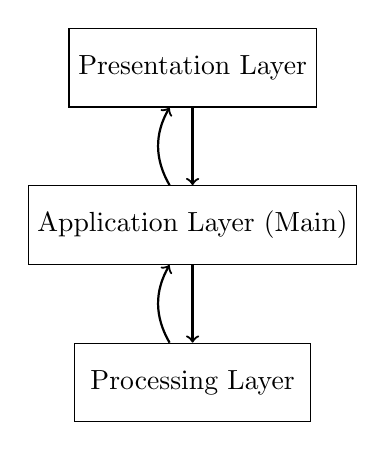
\begin{tikzpicture}
        \node[draw, rectangle, minimum width=3cm, minimum height=1cm] (UI) at (0,2) {Presentation Layer};
        \node[draw, rectangle, minimum width=3cm, minimum height=1cm] (App) at (0,0) {Application Layer (Main)};
        \node[draw, rectangle, minimum width=3cm, minimum height=1cm] (Proc) at (0,-2) {Processing Layer};
        
        \draw[->, thick] (UI) -- (App);
        \draw[->, thick] (App) -- (Proc);
        \draw[->, thick] (Proc) to[bend left] (App);
        \draw[->, thick] (App) to[bend left] (UI);
    \end{tikzpicture}
    
    \vspace{0.5cm}
    \footnotesize{Full diagram available in system documentation.}
\end{frame}

% Slide 14: UML State Chart
\begin{frame}{UML State Chart Diagram (FSM)}
    \centering
    \begin{tikzpicture}[node distance=2.5cm, auto]
        \node[draw, circle] (Start) {Start};
        \node[draw, rectangle, right of=Start] (Init) {Initializing};
        \node[draw, rectangle, right of=Init] (Monitor) {Monitoring};
        \node[draw, rectangle, below of=Monitor] (Paused) {Paused};
        \node[draw, rectangle, right of=Monitor] (Alert) {Alerting};
        
        \path[->] (Start) edge (Init);
        \path[->] (Init) edge (Monitor);
        \path[->] (Monitor) edge[bend left] (Paused);
        \path[->] (Paused) edge[bend left] (Monitor);
        \path[->] (Monitor) edge frequency (Alert);
    \end{tikzpicture}
    
    \vspace{0.5cm}
    \textbf{States:} 19 Defined States handling Flow settings, Errors, and Privacy commands.
\end{frame}

% Slide 15: Implementation Results - Interface
\begin{frame}{Implementation: The Interface}
    \textbf{Key Achievements:}
    \begin{itemize}
        \item \textbf{Latency:} End-to-end processing $<$ 50ms.
        \item \textbf{Responsiveness:} UI never freezes due to \texttt{QThread} offloading.
        \item \textbf{Feedback:} Immediate visual confirmation of state ("Searching" vs "Derived").
    \end{itemize}
\end{frame}

% Slide 16: Implementation Results - Smile Detection
\begin{frame}{Implementation: Reactive Smile Detection}
    \textbf{Algorithm:}
    \begin{enumerate}
        \item Extract Face ROI (Region of Interest).
        \item Apply Smile Haar Cascade with strict tuning (Neighbors=20).
        \item If \texttt{True} $\rightarrow$ Boost "Happy" probability $\rightarrow$ Update UI.
    \end{enumerate}
    
    \vspace{0.5cm}
    \textbf{Result:}
    A responsive interaction loop that encourages positive affect without complex deep learning models.
\end{frame}

% Slide 17: Conclusions
\begin{frame}{Conclusions \& Lessons Learnt}
    \textbf{Conclusions:}
    \begin{itemize}
        \item Successfully delivered a privacy-preserving desktop monitor.
        \item "Reactive" algorithms (e.g., smile detection) can effectively simulate complex emotion awareness.
    \end{itemize}
    
    \textbf{Lessons Learnt:}
    \begin{itemize}
        \item \textbf{Concurrency is Key:} Main thread must remain free for GUI rendering.
        \item \textbf{User Feedback:} Text labels ("Searching...") drastically reduce user confusion compared to silent failures.
    \end{itemize}
\end{frame}

% Slide 18: References
\begin{frame}{References}
    \footnotesize
    \begin{thebibliography}{99}
        \bibitem{ekman} Ekman, P. (1992). An argument for basic emotions. \textit{Cognition and Emotion}.
        \bibitem{calvo} Calvo, R. A., \& D'Mello, S. (2010). Affect detection. \textit{IEEE Transactions on Affective Computing}.
        \bibitem{viola} Viola, P., \& Jones, M. (2001). Rapid object detection using a boosted cascade of simple features. \textit{CVPR}.
        \bibitem{opencv} OpenCV Documentation. \url{https://opencv.org/}
    \end{thebibliography}
\end{frame}

\end{document}
